\documentclass{article}
\usepackage{amsmath}
\usepackage{graphicx}
\usepackage{epstopdf}
\usepackage{float}
\usepackage{subfigure}
\title{CSL603 - Machine Learning\\Lab 2}
\author{Aditya Gupta\\2015CSB1003}
\begin{document}
\maketitle
\section{Linear Ridge Regression}
Given $X$ and $Y$ we will find $W$ that minimizes $J(W)$, the error function and are defined as:
$$f(X)=
\underbrace{
\begin{pmatrix}
1&x_{11}&\cdots&x_{1D}\\
1&x_{21}&\cdots&x_{2D}\\
\vdots&\vdots&\ddots&\vdots\\
1&x_{N1}&\cdots&x_{ND}
\end{pmatrix}}_{X}
\underbrace{
\begin{pmatrix}
w_0\\w_1\\\vdots\\w_D
\end{pmatrix}}_{W}
=
\underbrace{
\begin{pmatrix}
y_0\\y_1\\\vdots\\y_N
\end{pmatrix}}_{Y}$$
$$
\min_W J(W)\equiv\min_W\frac12(XW-Y)^T(XW-Y)+\frac12\lambda||W||^2
$$
Which when solved gives us:
$$W=(X^TX+\lambda I)^{-1}X^TY$$
\subsection*{Observations}
The following observations were obtained:
\begin{itemize}

\begin{figure}[H]
\makebox[\textwidth][c]{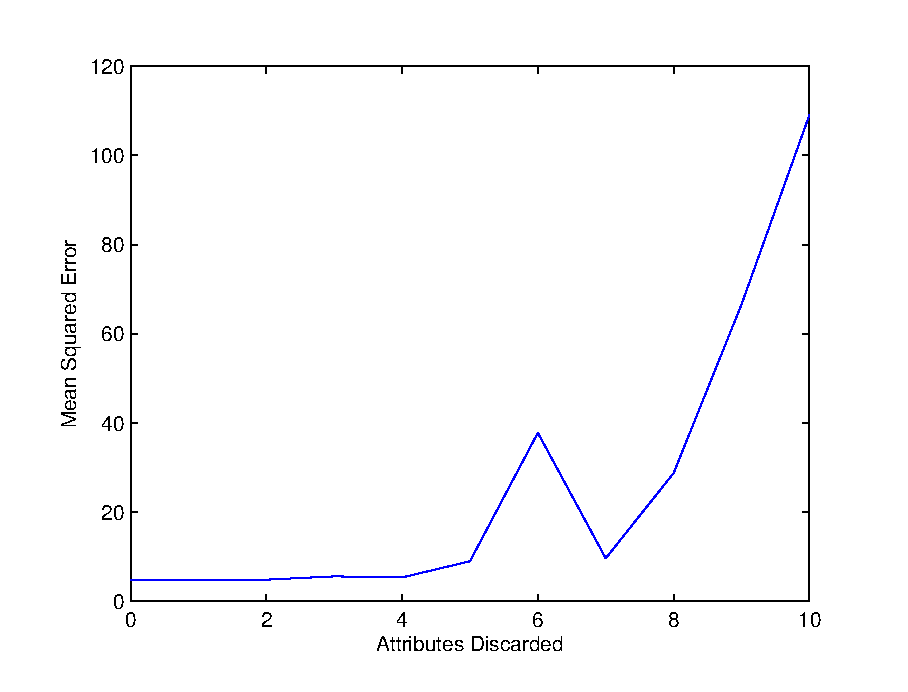
\includegraphics{fig6.eps}}
 \caption{Mean Sqaured Error for after discarding increasing number of least significant weights in $W$.}
 \label{fig:1}
 \end{figure}
 
\item A particular value of $\lambda$(say $0$) was choosen and then the magnitude of entries in the weights $W$ was compared and one by one the least significant ones were discarded and the mean squared error changes can be seen in Figure \ref{fig:1}. We can see that discarding 2-4 least significant attributes does not make any major change to the mean squared error, hence we can conclude that the input data contained some attributes that were irrelevant in estimating the output values.

\begin{figure}[H]
\makebox[\textwidth][c]{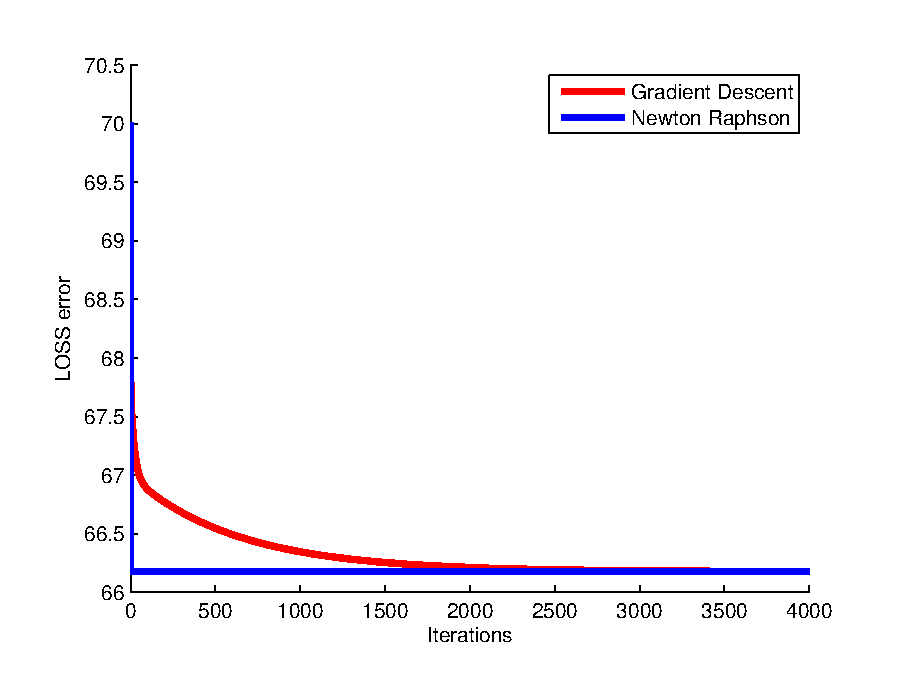
\includegraphics[scale=0.65]{fig1.eps}}
 \caption{Average Mean Sqaured Error for various values of training set fraction and $\lambda$ values used in Ridge Regression for Training Data.}
 \label{fig:2}
 \end{figure}

 \begin{figure}[H]
\makebox[\textwidth][c]{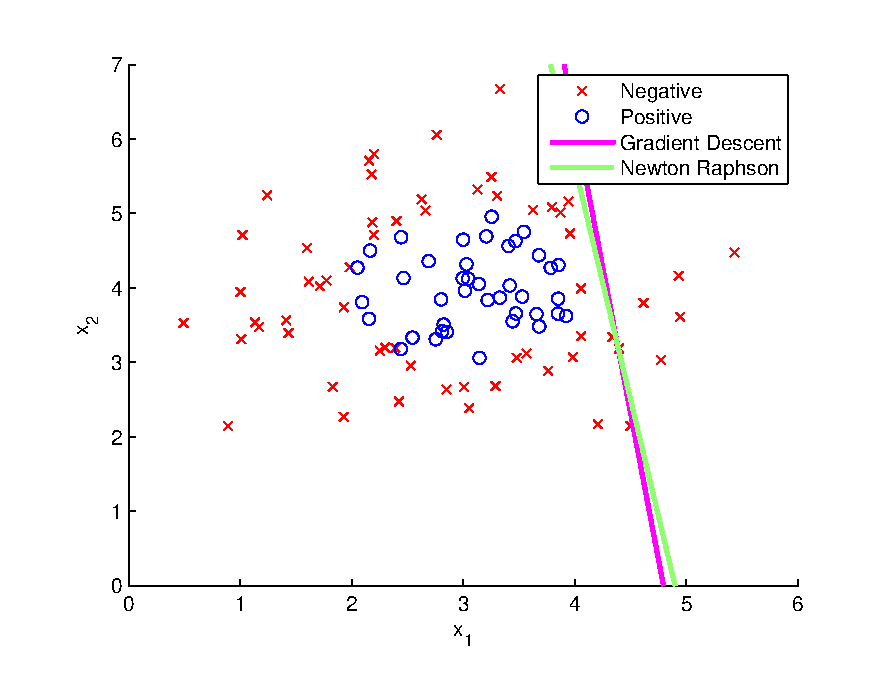
\includegraphics[scale=0.65]{fig2.eps}}
 \caption{Average Mean Sqaured Error for various values of training set fraction and $\lambda$ values used in Ridge Regression for Testing Data.}
 \label{fig:3}
 \end{figure}

\item The effect of $\lambda$ on error was observed for different partitions of the data into training and testing sets. The average mean sqaured error for 100 repetitions for splitting-fractions varying from $1\%$ to $99\%$ and lambda values from $0$ to $100$ was observed. The surface corresponding to the average mean absolute error can be seen in Figure \ref{fig:2} and \ref{fig:3}. We can see that for low values of training set fraction or high $\lambda$ values the average mean squared error increased quite a bit.
 
 \begin{figure}[H]
\makebox[\textwidth][c]{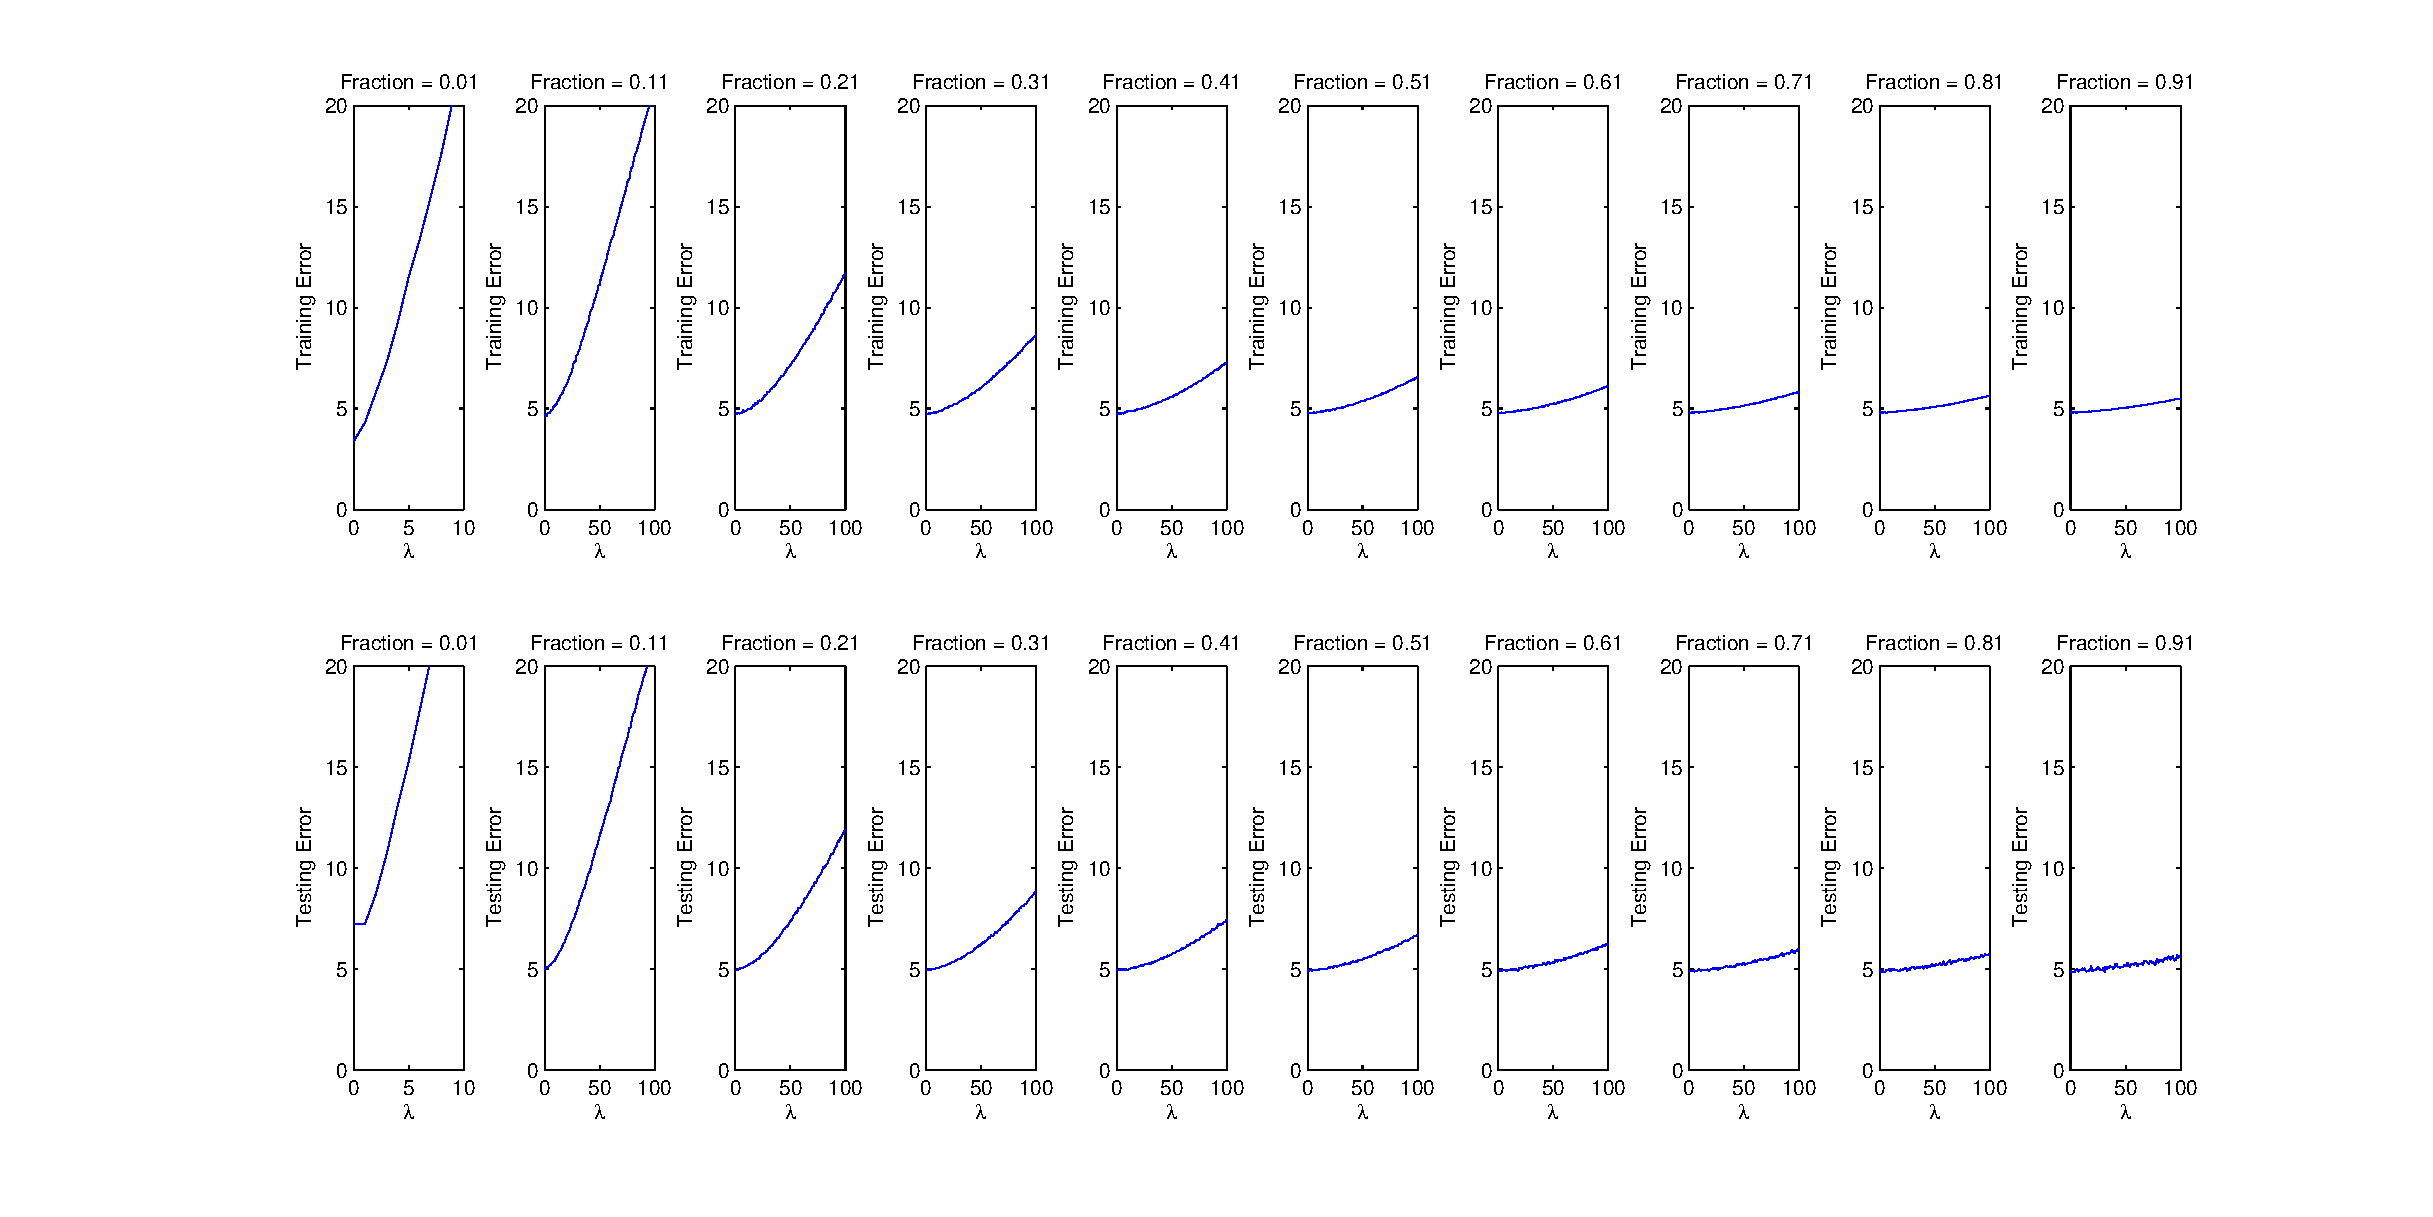
\includegraphics[scale=0.7]{fig3.eps}}
 \caption{Average Mean Squared Error for various training set fractions varying against the $\lambda$ values}
 \label{fig:4}
 \end{figure}
 
\item Figure \ref{fig:2} and \ref{fig:3}'s surfaces can be plotted into different graphs for few particular values of splitting-fractions and varying lambda and obsreving the change in average mean absolute error. Figure \ref{fig:4} shows that for high $\lambda$ values the average mean squared error increases and is shaped like a convex function and the increase is more apparent in low training set fraction values.

\begin{figure}[H]
\makebox[\textwidth][c]{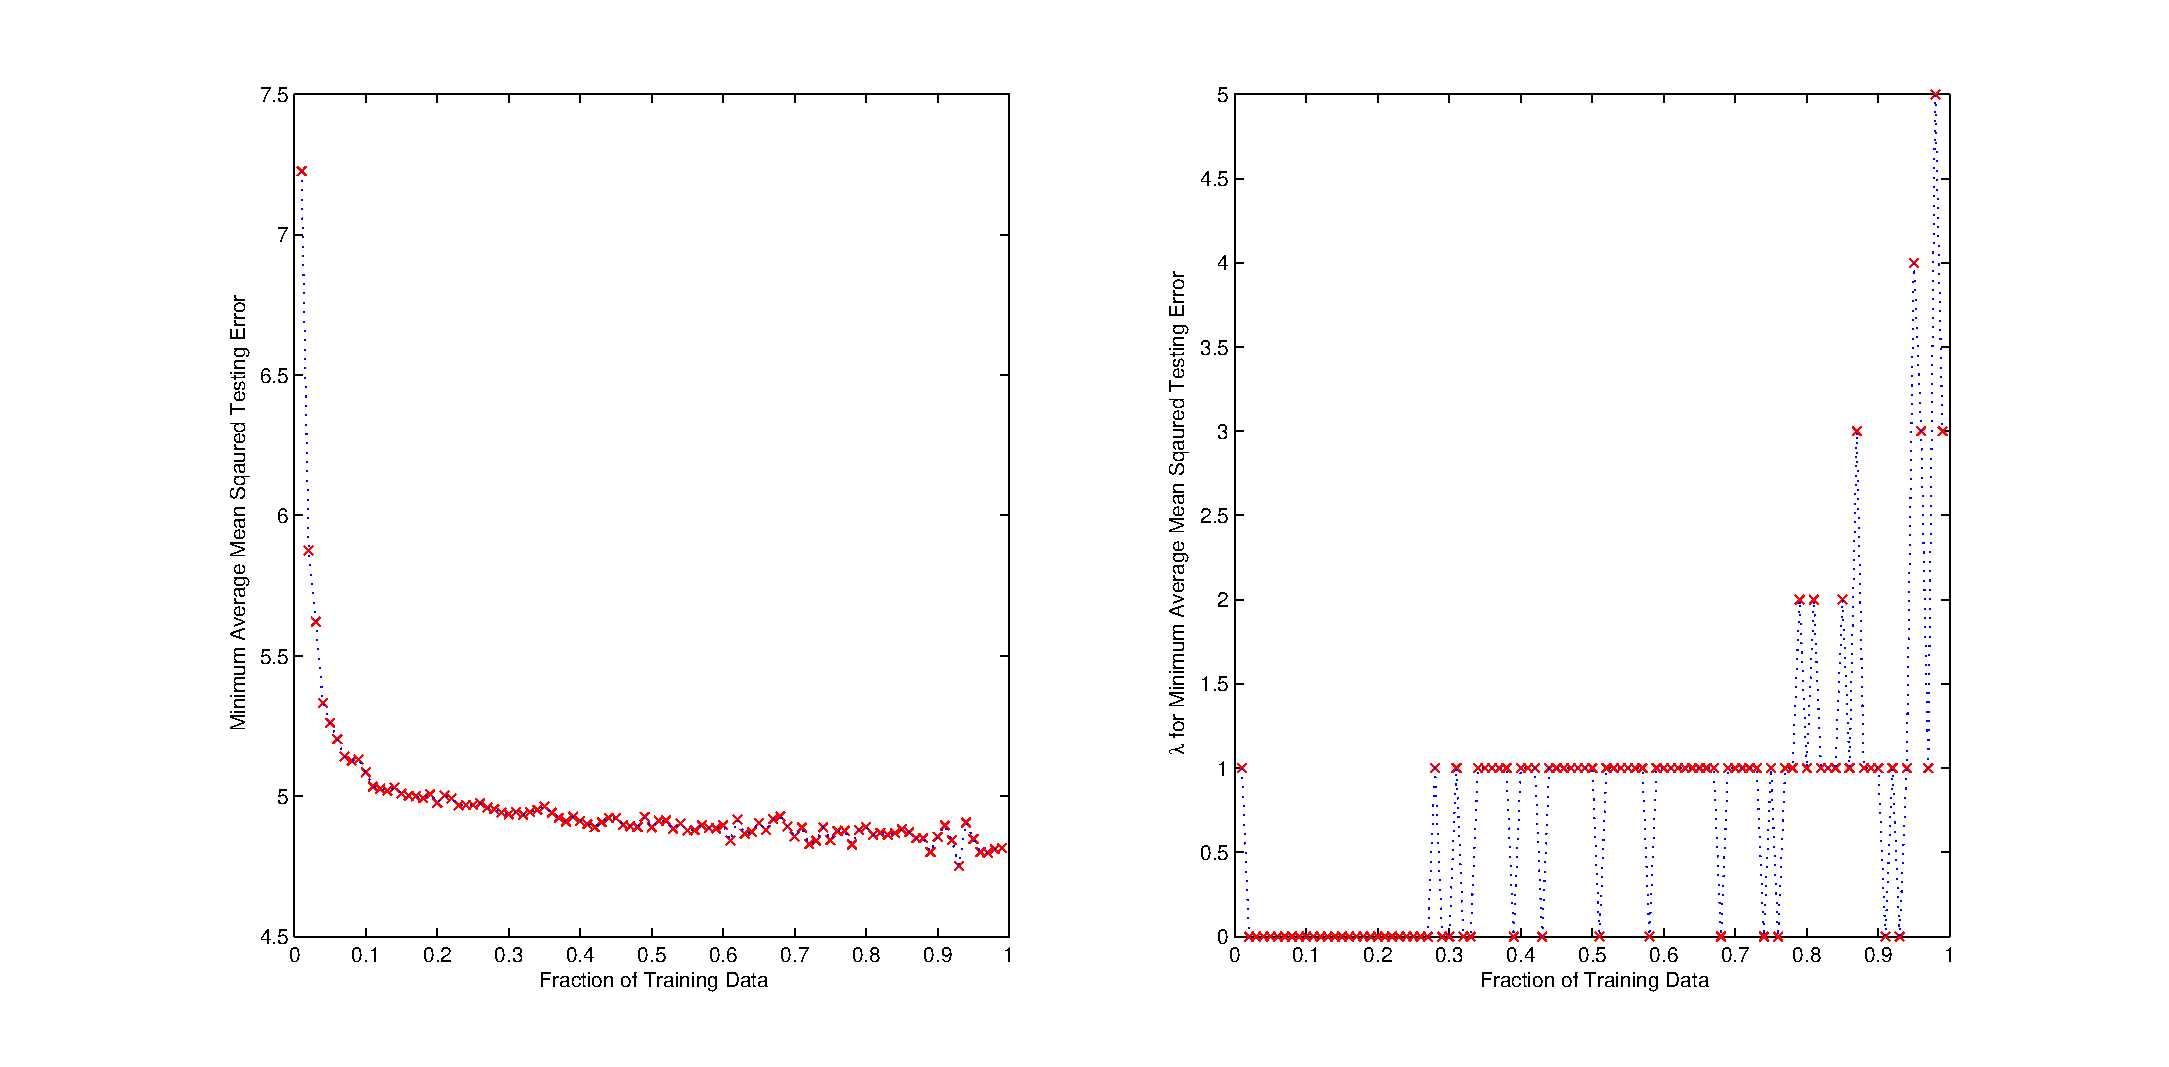
\includegraphics[scale=0.7]{fig4.eps}}
 \caption{Minimum Average Mean Squared Error for various values of training set fraction and the corresponding $\lambda$ values.}
 \label{fig:5}
 \end{figure}

\item Now we noted the minimum average mean squared testing error for each training set fraction values. Also the corresponding $\lambda$ value was observed. We can see from Figure \ref{fig:5} that with high taining set fraction the minimum average mean sqaured error decreases and though the $\lambda$ values at which these values are obtained  in general have higher magnitude ($\lambda$) as we increase the training set fraction, we can say that probably the model is overfitting and to penalize it we need higher magnitude of $\lambda$.

\begin{figure}[H]
\makebox[\textwidth][c]{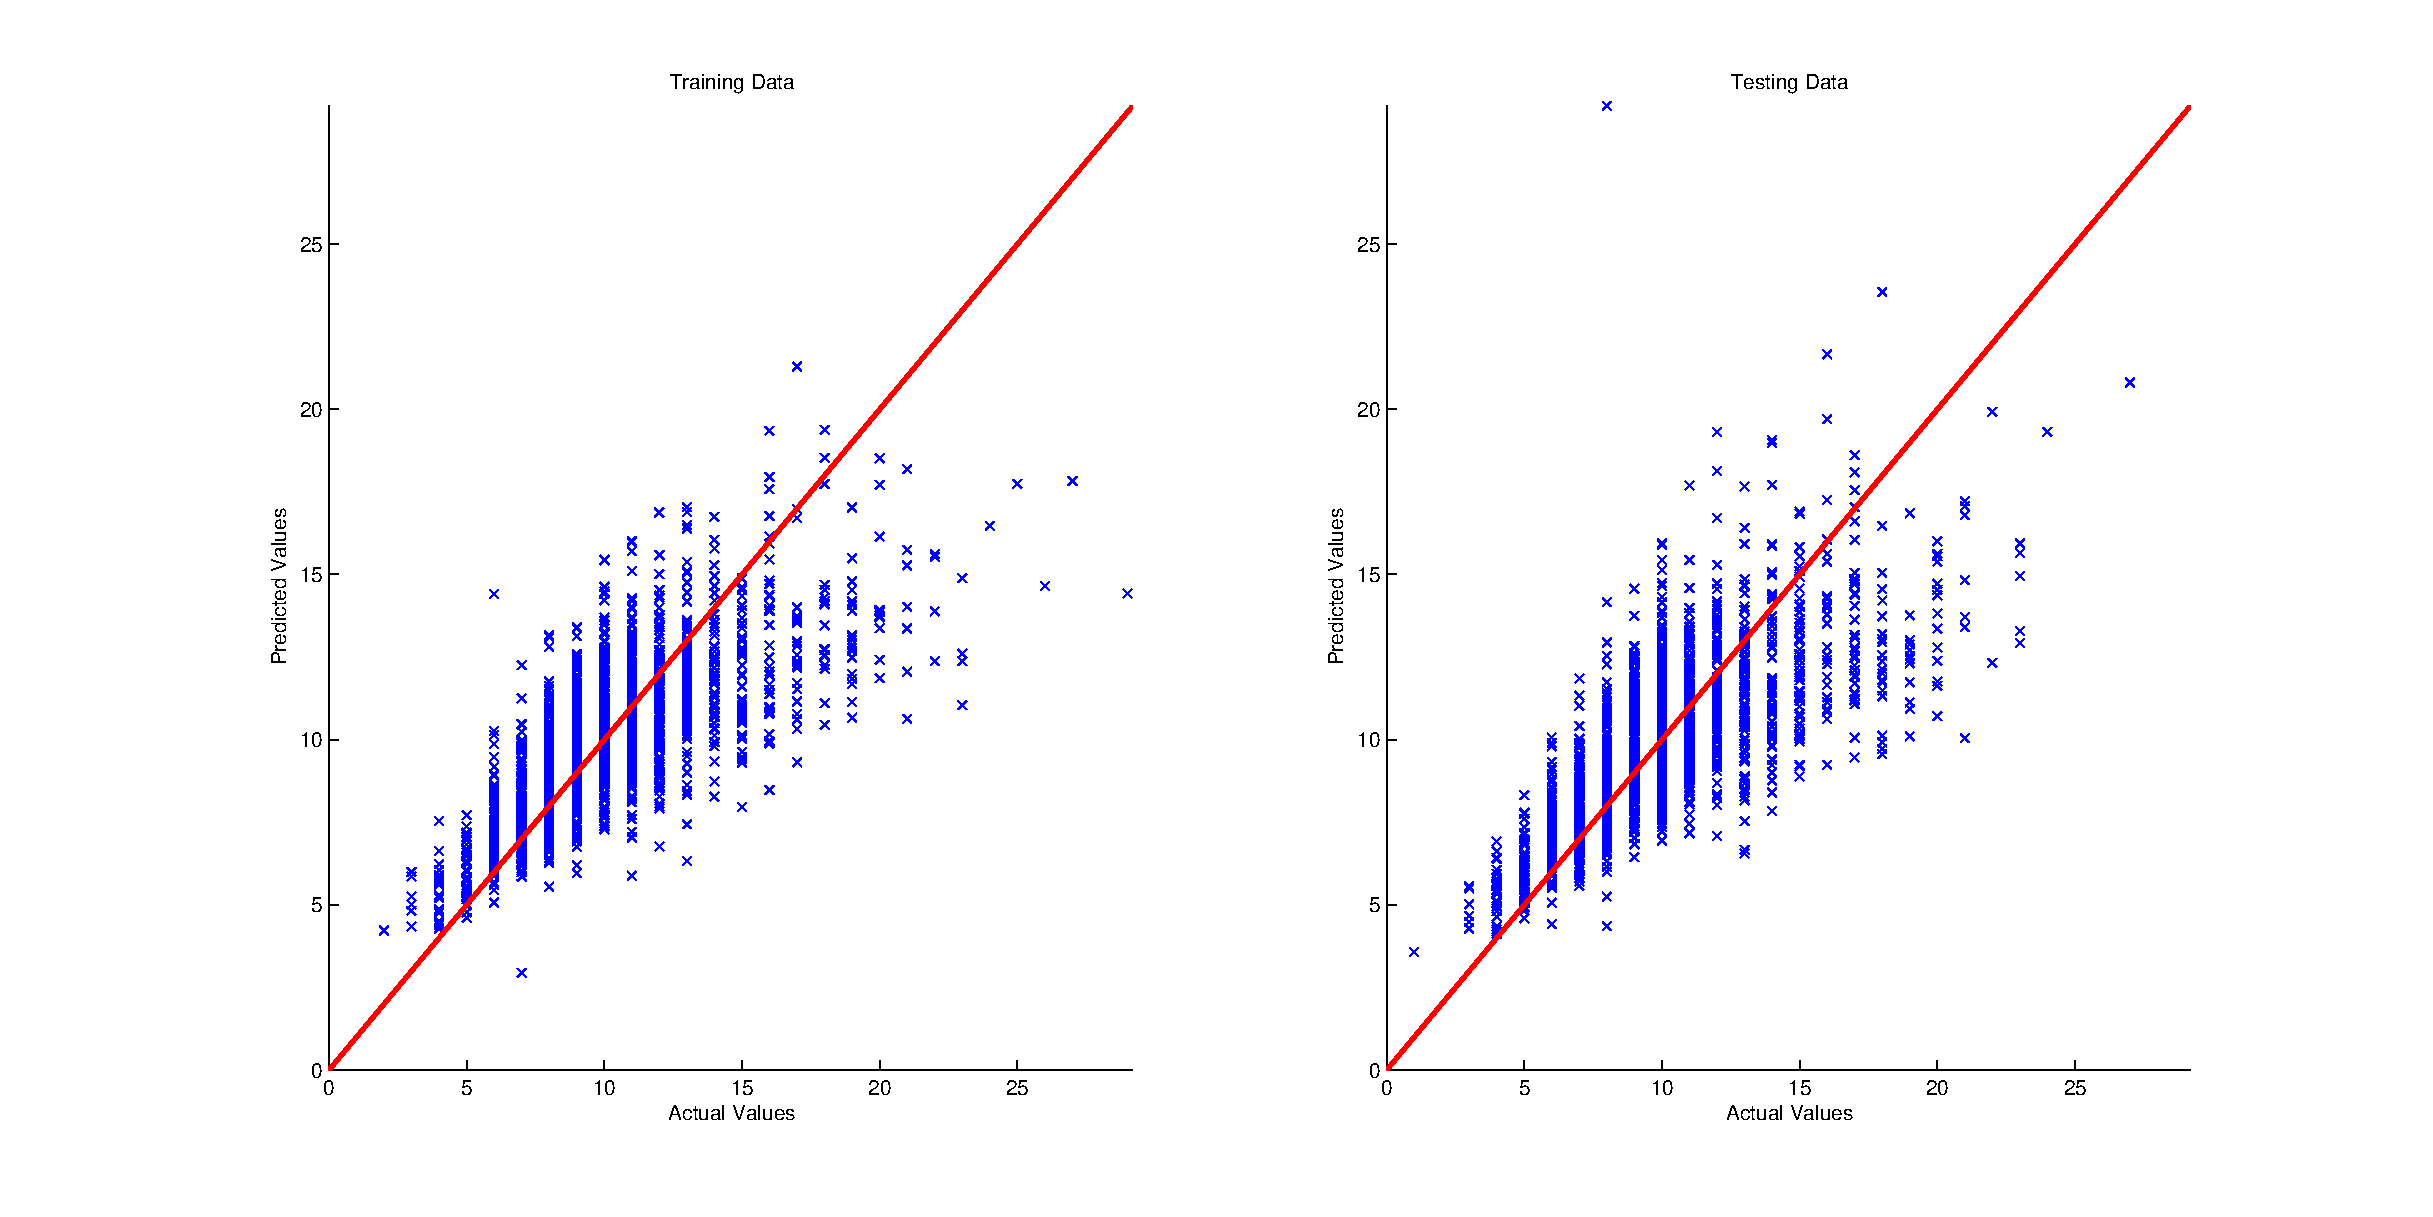
\includegraphics[scale=0.7]{fig5.eps}}
 \caption{Relation between the actual data set values and predicted values for training and testing data. The reference line $y=x$ is shown in red.}
 \label{fig:6}
 \end{figure}
 
\item The correspondence between the actual and predicted values was also observed. For perfect prediction, this should correspond to a straight line through origin at $45^\circ$ degrees. Figure \ref{fig:6} shows that the actual values and the predicted values lie close to the line $y=x$ thus ensuring that there is a significant correlation and accuracy to the predicted values.
 
\end{itemize}

\subsection*{Summary: Conclusions}
\begin{itemize}
\item {\bf Underfitting}: With high $\lambda$ values the average mean squared error increases.
\item {\bf Decrease in Variance}: With high training set fraction the average mean squared error decreases.
\item {\bf Correctness of the Model}: The actual and predicted values lie quite close to the line $y=x$.
\item {\bf Redundant Attributes}: Discarding few attributes doesn't make quite a difference hence their irrelevancy to the use in prediction of output values.
\end{itemize}

\section{Regularized Logistic Regression}
Given $x_1$ and $x_2$ attribute values for different individual whether the credit card application should be accepted or rejected.
\begin{itemize}

\begin{figure}[H]
\makebox[\textwidth][c]{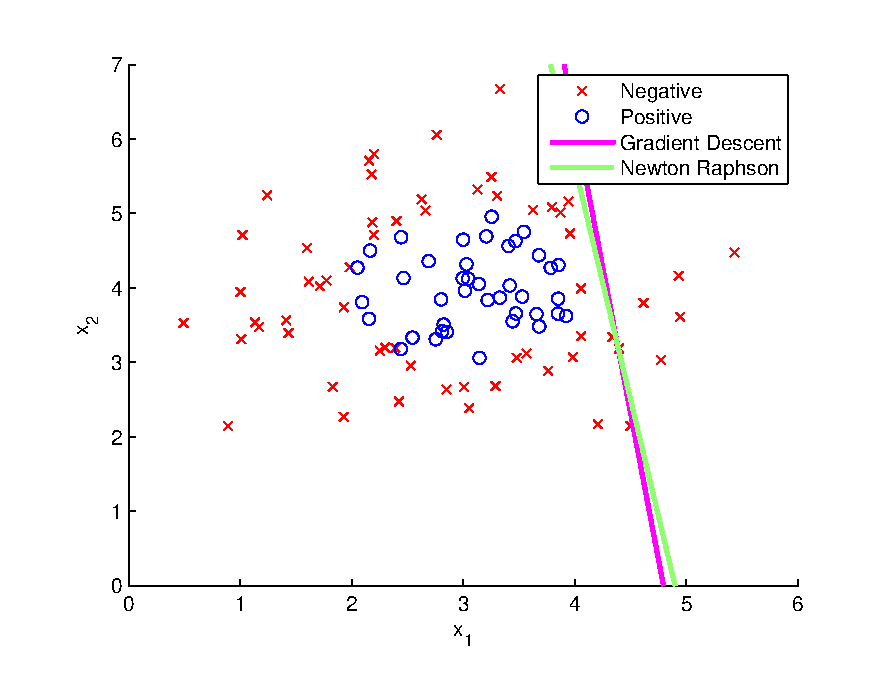
\includegraphics[scale=1]{fig2_2.eps}}
 \caption{Distribution of the dataset, the positive examples are in blue circles and negative examples in red crossed. The magenta line represents the class boundary obtained using gradient descent (linear classification), similarly the green one for Newton Raphson method.}
 \label{fig:7}
 \end{figure}
 
 \item As we know:
 $$\sigma(\theta) = \frac1{1+e^{-\theta}}$$
 $$f(x_i)=\sigma\left(\sum_{d=1}^Dw_ix_{id}\right)$$
 $$J(w)=-\sum_{i=1}^N[y_i\log(f(x_i))+(1-y_i)\log(1-f(x_i))]$$
 We obtain:
 $$\nabla_wJ(w)=X^T({\bf F}(X)-{\bf Y})$$
 Hence, for Gradient Descent:
 $$w'=w-\alpha X^T({\bf F}(X)-{\bf Y})$$
 and for Newton Raphson:
 $$w' = w-H^{-1}\nabla J(w)$$
 where
 $$H=X^TRX\; R=\text{diag}(f(x_1)(1-f(x_1)), f(x_2)(1-f(x_2)), ...)$$
 so:
 $$w' = w - (X^TRX)^{-1}({\bf F}(X)-{\bf Y})$$
 
\item The dataset plotted can be seen in Figure \ref{fig:7}. It can be seen that the data is not linearly separable and hence both gradient descent and newton raphson do not classify it properly.

\begin{figure}[H]
\makebox[\textwidth][c]{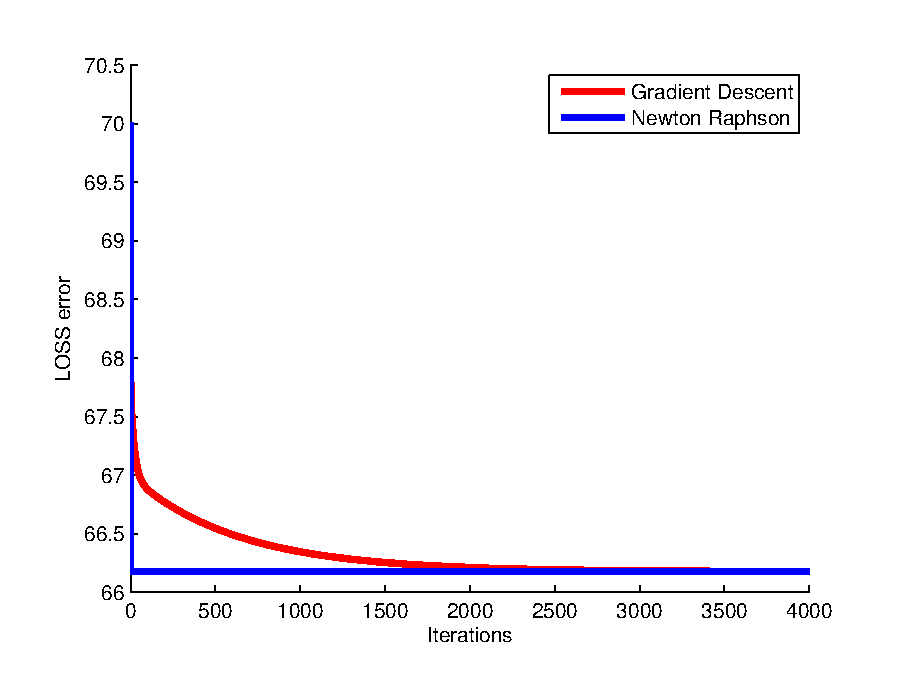
\includegraphics[scale=1]{fig1_2.eps}}
 \caption{The loss error in prediction of classes by gradient descent and newton raphson methods using linear classification as a function of number of iterations.}
 \label{fig:8}
 \end{figure}
 
 \item Both the methods reach at almost the same solution. The number of iterations required by Gradient Descent is however large ($\sim2000$) as compared to Newton Raphson ($\sim10$) as seen in Figure \ref{fig:8}.
 
 \item We can perform feature transformation to map $x_1, x_2$ to higher degree polynomials, then we obtain the Figures \ref{fig:9}, \ref{fig:10}, \ref{fig:11} and \ref{fig:12}.
 
 \begin{figure}[H]
\makebox[\textwidth][c]{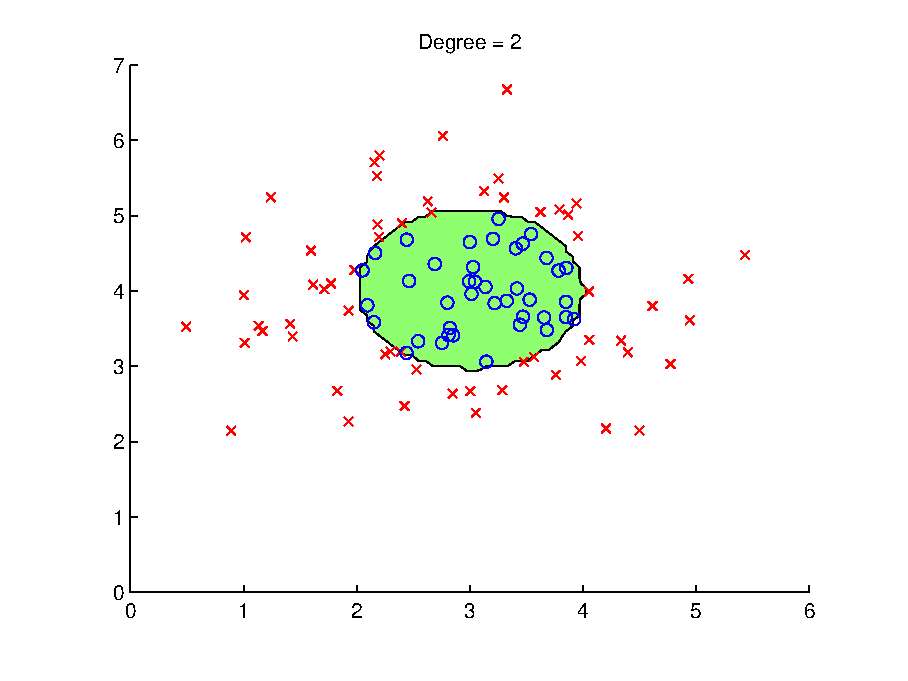
\includegraphics[scale=0.7]{d2l0f2.eps}}
 \caption{Plot of classification boundary for degree 2.}
 \label{fig:9}
 \end{figure}
 
  \begin{figure}[H]
\makebox[\textwidth][c]{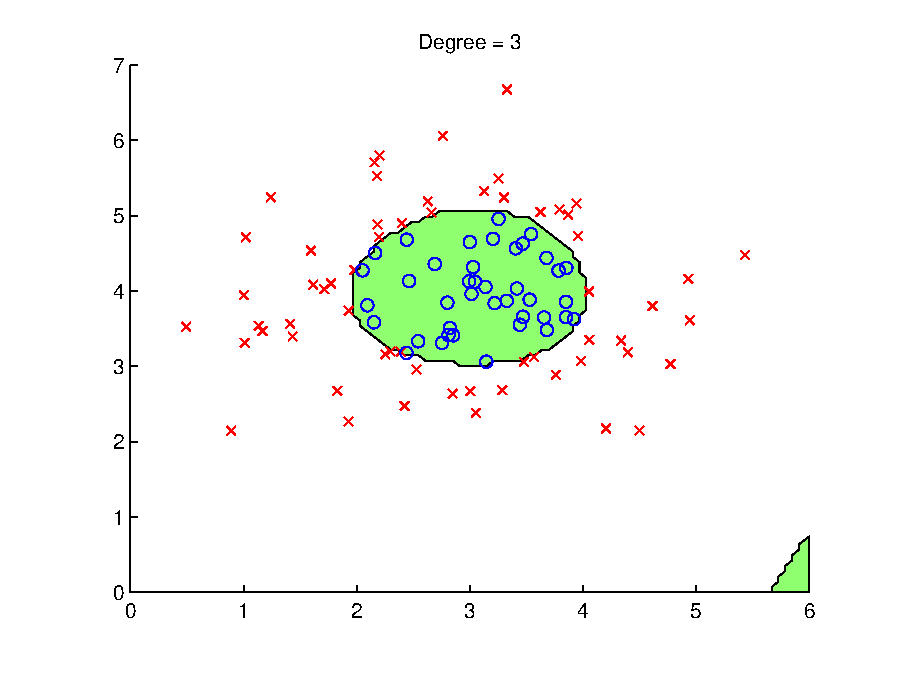
\includegraphics[scale=0.7]{d3l0f2.eps}}
 \caption{Plot of classification boundary for degree 3.}
 \label{fig:10}
 \end{figure}
 
  \begin{figure}[H]
\makebox[\textwidth][c]{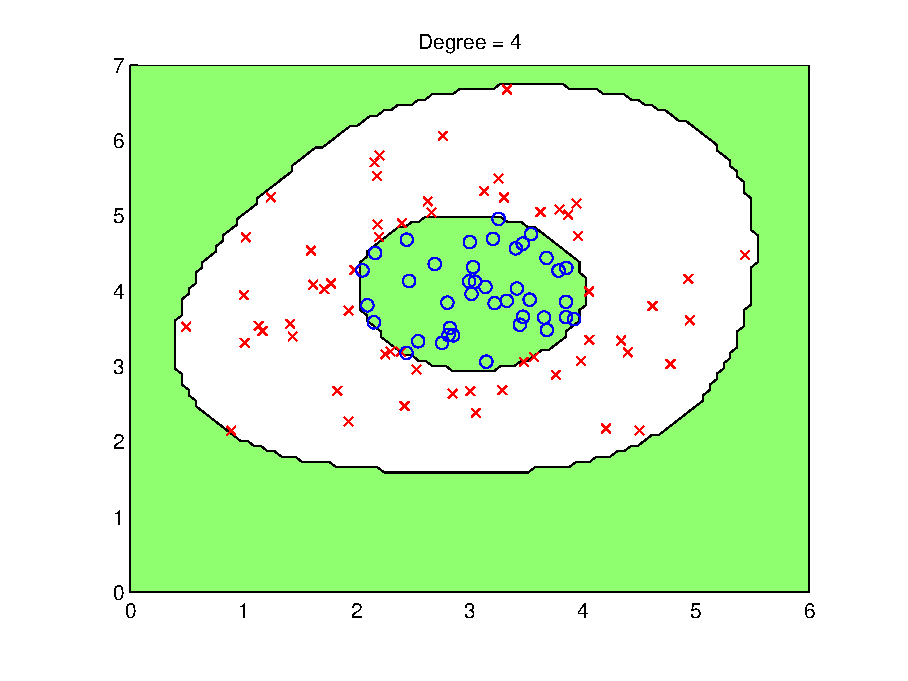
\includegraphics[scale=0.7]{d4l0f2.eps}}
 \caption{Plot of classification boundary for degree 4.}
 \label{fig:11}
 \end{figure}
 
   \begin{figure}[H]
\makebox[\textwidth][c]{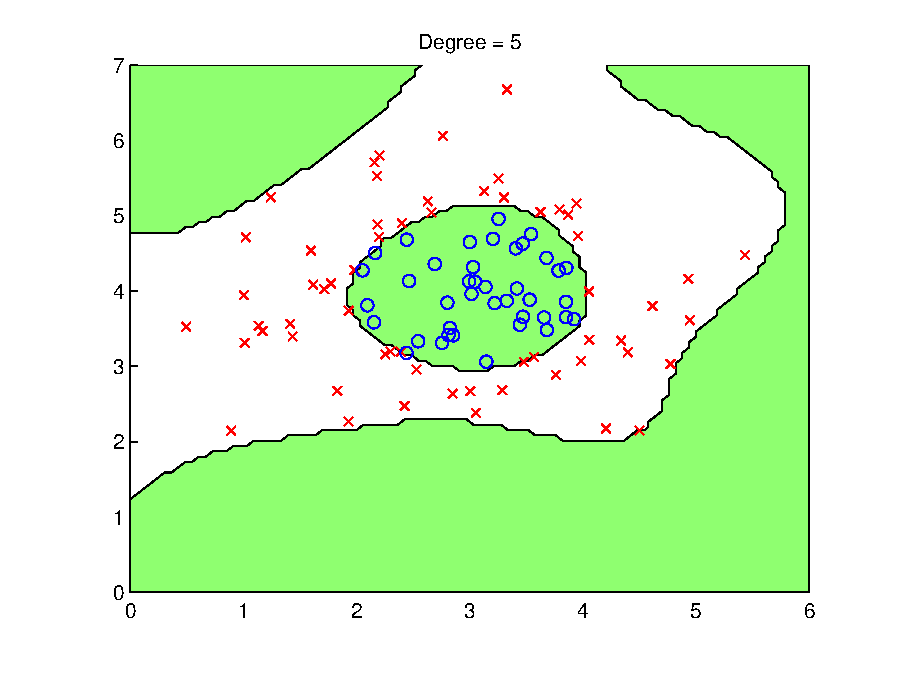
\includegraphics[scale=0.7]{d5l0f2.eps}}
 \caption{Plot of classification boundary for degree 5.}
 \label{fig:12}
 \end{figure}
 
 \item We can also introduce a regularization parameter $\lambda$ that will modify our equations in the following way:
 $$J(w)=-\sum_{i=1}^N[y_i\log(f(x_i))+(1-y_i)\log(1-f(x_i))]+\frac \lambda 2||w||^2$$
 $$\nabla_wJ(w)=X^T({\bf F}(X)-{\bf Y})+\lambda w$$
For Newton Raphson:
 $$w' = w-H^{-1}\nabla J(w)$$
 where
 $$H=X^TRX+\lambda I$$
 so:
 $$w' = w - (X^TRX+\lambda I)^{-1}({\bf F}(X)-{\bf Y}+\lambda w)$$
 \item Some examples of figures then obtained are Figure \ref{fig:13} and \ref{fig:14}. These boundaries underfit the given data but have simpler weights.
 
    \begin{figure}[H]
\makebox[\textwidth][c]{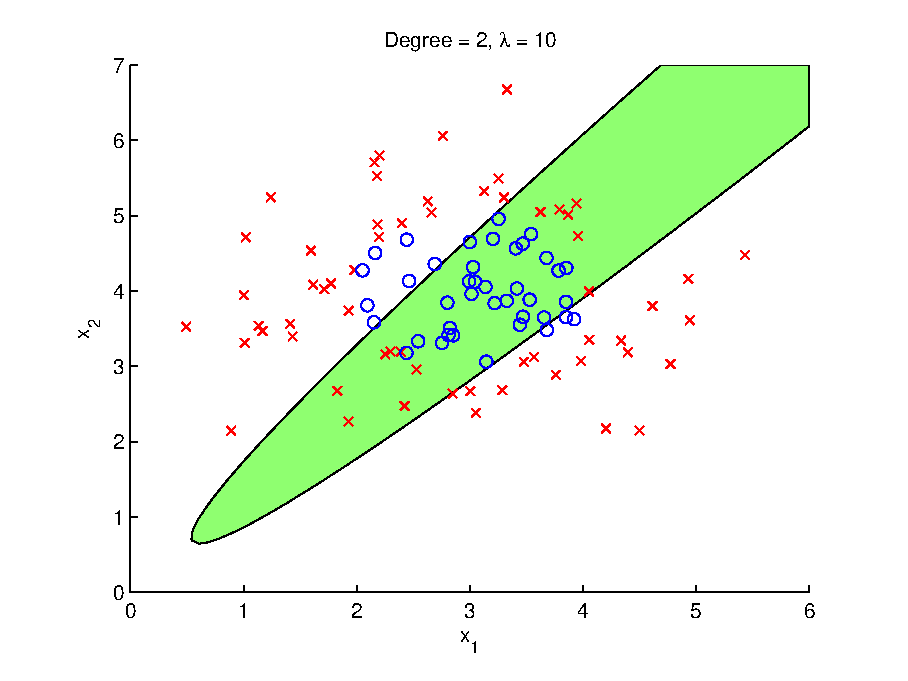
\includegraphics[scale=1]{d2l10f2.eps}}
 \caption{Plot of classification boundary for degree 2 ($\lambda=10$).}
 \label{fig:13}
 \end{figure}
     \begin{figure}[H]
\makebox[\textwidth][c]{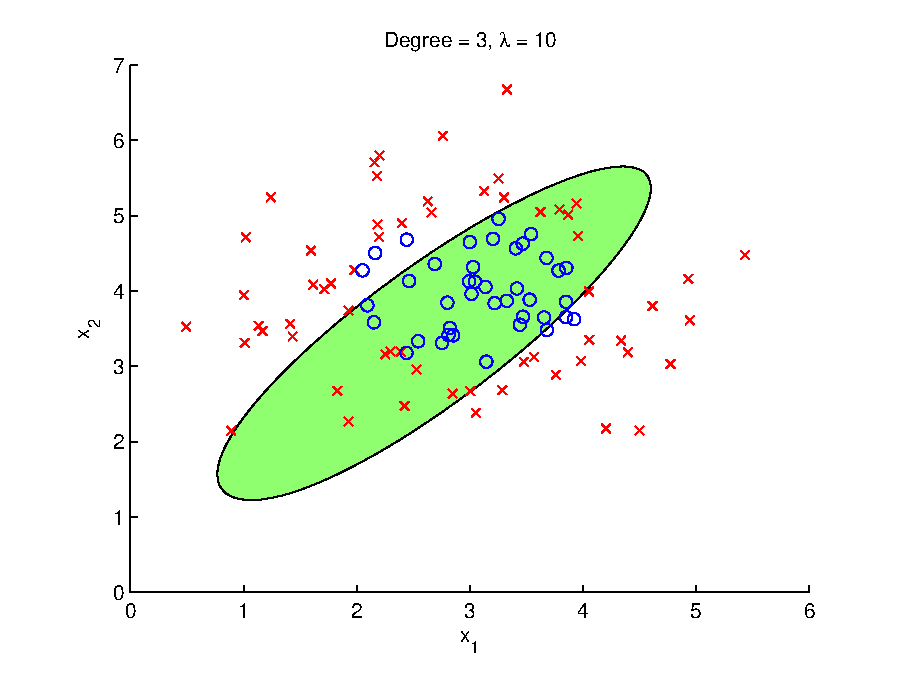
\includegraphics[scale=1]{d3l10f2.eps}}
 \caption{Plot of classification boundary for degree 3 ($\lambda=10$).}
 \label{fig:14}
 \end{figure}
 
 \item Now we divide the given data (we generate 1000 points using \verb|l2reglog.m| with introducing 10\% noise) into training and testing sets (50\% - 50\%) and check for overfitting and underfitting. The following appropriate figures were obtained.
 
     \begin{figure}[H]
\makebox[\textwidth][c]{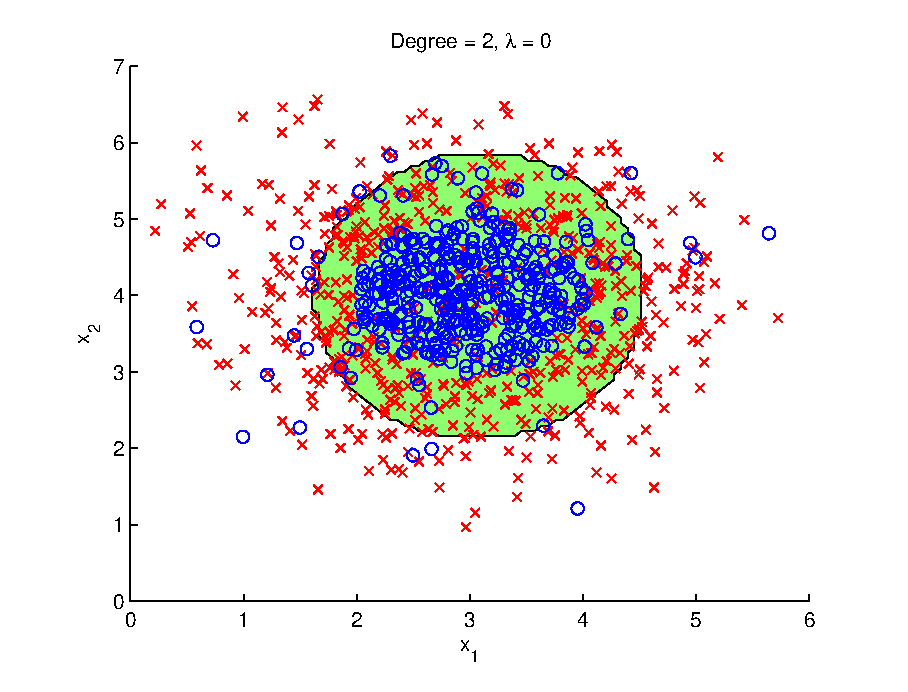
\includegraphics[scale=1]{d2l0f2_c2.eps}}
 \caption{Plot of classification boundary for degree 2 ($\lambda=0$) overfitting the data.}
 \label{fig:13}
 \end{figure}
     \begin{figure}[H]
\makebox[\textwidth][c]{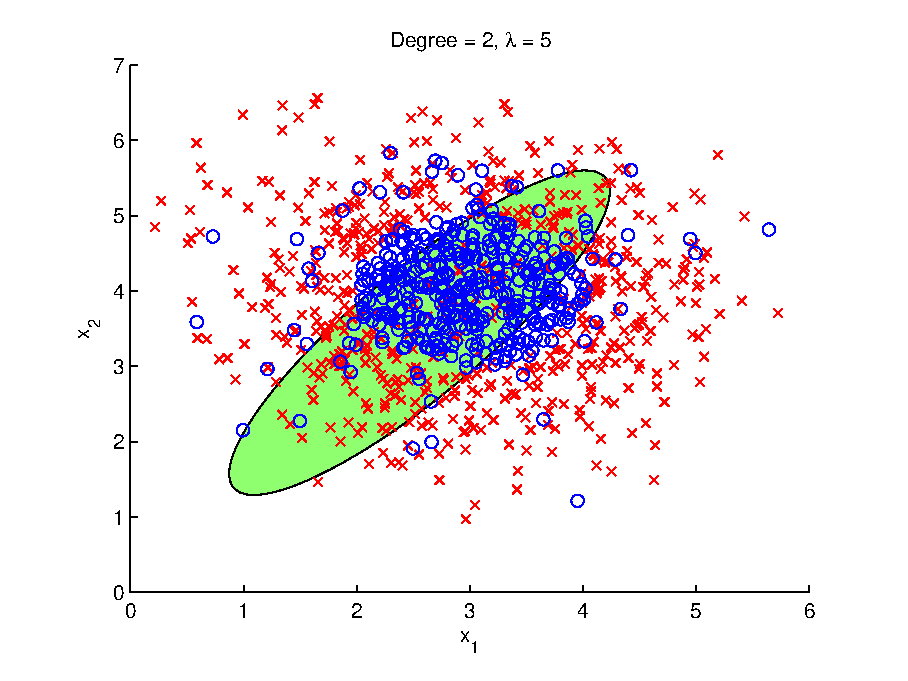
\includegraphics[scale=1]{d2l5f2_c2.eps}}
 \caption{Plot of classification boundary for degree 2 ($\lambda=10$) underfitting the data.}
 \label{fig:14}
 \end{figure}
\end{itemize}
\end{document}